\section{E-Mail}
\begin{frame}{Was soll geschützt werden?}
  E-Mails können
  \begin{itemize}
    \item abgehört
    \item gefälscht
  \end{itemize}
  werden. \pause Deshalb stellen wir vor, wie man
  \begin{itemize}
    \pause
    \item die Vertraulichkeit (das ,,Briefgeheimnis``) umsetzt
    \\ $\Rightarrow$ Verschlüsselung
    \pause
    \item die Echtheit des Gegenübers sicherstellt
    \\ $\Rightarrow$ Digitale Signatur
  \end{itemize}
  \pause
  \vfill
  Außerdem:\\ Wie man sicherstellt, dass das E-Mail Passwort\\ nicht einfach mitgelesen werden kann
\end{frame}

\renewcommand{\emailtext}{Von: Alice@provider1.de\\An: Bob@provider2.com\\Betreff: Hallo\\Hallo Bob, wie gehts dir?\\LG Alice}
\renewcommand{\emailciphertext}{Von: Alice@provider1.de\\An: Bob@provider2.com\\Betreff: Hallo\\\colorbox{blue}{\parbox[t][1.2em][t]{.88\messagewidth}{~}}}
\settowidth{\messagewidth}{\tiny Hallo Bob, wie gehts dir?}
\addtolength{\messagewidth}{3\pgfkeysvalueof{/pgf/outer xsep}}

\begin{frame}{Funktionsweise}
  \framezoom<1><2>(-0.3cm,0cm)(3cm,4.5cm)
  \framezoom<1><3>(4.5cm,0cm)(3cm,4.5cm)
  \begin{center}\tiny
  \begin{tikzpicture}[align=left]
    \tikzstyle{attacker} = [draw,circle]
    \tikzstyle{entity} = [draw,rectangle split,rectangle split parts=2]
    \tikzstyle{message} = [fill=white,text width=\messagewidth]
      \node[attacker] (eve) at (0,0) {Eve};
      \node[entity] (alice) at (-3.75cm,2.5cm) {Alice\nodepart{second}\emailtext};
      \node[entity] (Palice) at (-3.75cm,-2.0cm) {provider1.de\nodepart{second}\emailtext};
      \node[entity] (Pbob) at (3.75cm,-2.0cm) {provider2.com\nodepart{second}\emailtext};
      \node[entity] (bob) at (3.75cm,2.5cm) {Bob\nodepart{second}\emailtext};
      \draw[->] (alice) -- (Palice) node [pos=0.25,message] (aliceHello) {Hier ist Alice, mein Passwort ist AAA. Ich will eine E-Mail verschicken:} node [pos=0.70,message] (aliceSend) {\emailtext};
      \draw[->] (Palice) -- (Pbob) node [midway,message] (providerFwd) {\emailtext};
      \draw[<->] (bob) -- (Pbob) node [pos=0.25,message] (bobHello) {Hier ist Bob, mein Passwort ist BBB. Gib mir meine neuen E-Mails!} node [pos=0.70,message] (bobReceive) {\emailtext};
      \foreach \t in {(aliceHello),(aliceSend),(Palice),(providerFwd),(Pbob),(bobHello),(bobReceive)} \draw[->,red,thick] (eve) -- \t;
      \draw[dashed,red] ($ (alice.south west)!.5!(aliceHello.north west) $) -- ($ (bob.south east)!.5!(bobHello.north east) $);
  \end{tikzpicture}
  \end{center}
  \vspace{-1em}
  \begin{itemize}
    \item \glqq Von\grqq\ und \glqq An\grqq\ kann Absender beliebig setzen,\\ wie auf einem Briefumschlag!
  \end{itemize}
\end{frame}

\begin{frame}{Transportverschlüsselung}{SSL/TLS, besser STARTTLS}
  \begin{center}\tiny
  \begin{tikzpicture}[align=left]
    \tikzstyle{attacker} = [draw,circle]
    \tikzstyle{entity} = [draw,rectangle split,rectangle split parts=2]
    \tikzstyle{message} = [fill=yellow,text=yellow,text width=\messagewidth]
      \node[attacker] (eve) at (0,0) {Eve};
      \node[entity] (alice) at (-3.75cm,2.5cm) {Alice\nodepart{second}\emailtext};
      \node[entity] (Palice) at (-3.75cm,-2.0cm) {provider1.de\nodepart{second}\emailtext};
      \node[entity] (Pbob) at (3.75cm,-2.0cm) {provider2.com\nodepart{second}\emailtext};
      \node[entity] (bob) at (3.75cm,2.5cm) {Bob\nodepart{second}\emailtext};
      \draw[->] (alice) -- (Palice) node [pos=0.25,message] (aliceHello) {Hier ist Alice, mein Passwort ist AAA. Ich will eine E-Mail verschicken:} node [pos=0.70,message] (aliceSend) {\emailtext};
      \draw[->] (Palice) -- (Pbob) node [midway,message] (providerFwd) {\emailtext};
      \draw[<->] (bob) -- (Pbob) node [pos=0.25,message] (bobHello) {Hier ist Bob, mein Passwort ist BBB. Gib mir meine neuen E-Mails!} node [pos=0.70,message] (bobReceive) {\emailtext};
      \foreach \t in {(aliceHello),(aliceSend),(Palice),(providerFwd),(Pbob),(bobHello),(bobReceive)} \draw[->,red,thick] (eve) -- \t;
      \draw[dashed,red] ($ (alice.south west)!.5!(aliceHello.north west) $) -- ($ (bob.south east)!.5!(bobHello.north east) $);
  \end{tikzpicture}
  \end{center}
  \vspace{-1em}
  \begin{itemize}
    \item Inzwischen von fast allen Mailanbietern unterstützt
    \item Konfiguration des Mailprogramms überprüfen!
  \end{itemize}
\end{frame}

\begin{frame}{Ende-zu-Ende-Verschlüsselung}{OpenPGP, S/MIME}
  \begin{center}\tiny
  \begin{tikzpicture}[align=left]
    \tikzstyle{attacker} = [draw,circle]
    \tikzstyle{entity} = [draw,rectangle split,rectangle split parts=2]
    \tikzstyle{message} = [fill=white,text width=\messagewidth]
      \node[attacker] (eve) at (0,0) {Eve};
      \node[entity] (alice) at (-3.75cm,2.5cm) {Alice\nodepart{second}\emailtext};
      \node[entity] (Palice) at (-3.75cm,-2.0cm) {provider1.de\nodepart{second}\emailciphertext};
      \node[entity] (Pbob) at (3.75cm,-2.0cm) {provider2.com\nodepart{second}\emailciphertext};
      \node[entity] (bob) at (3.75cm,2.5cm) {Bob\nodepart{second}\emailtext};
      \draw[->] (alice) -- (Palice) node [pos=0.25,message] (aliceHello) {Hier ist Alice, mein Passwort ist AAA. Ich will eine E-Mail verschicken:} node [pos=0.70,message] (aliceSend) {\emailciphertext};
      \draw[->] (Palice) -- (Pbob) node [midway,message] (providerFwd) {\emailciphertext};
      \draw[<->] (bob) -- (Pbob) node [pos=0.25,message] (bobHello) {Hier ist Bob, mein Passwort ist BBB. Gib mir meine neuen E-Mails!} node [pos=0.70,message] (bobReceive) {\emailciphertext};
      \foreach \t in {(aliceHello),(aliceSend),(Palice),(providerFwd),(Pbob),(bobHello),(bobReceive)} \draw[->,red,thick] (eve) -- \t;
      \draw[dashed,red] ($ (alice.south west)!.5!(aliceHello.north west) $) -- ($ (bob.south east)!.5!(bobHello.north east) $);
  \end{tikzpicture}
  \end{center}
  \vspace{-1em}
  \begin{itemize}
    \item Unabhängig vom Mailanbieter möglich
    \item Benötigt Zusatzsoftware und Schlüssel bei beiden
  \end{itemize}
\end{frame}

\begin{frame}{Kombination Transport \& Ende-zu-Ende}
  \begin{center}\tiny
  \begin{tikzpicture}[align=left]
    \tikzstyle{attacker} = [draw,circle]
    \tikzstyle{entity} = [draw,rectangle split,rectangle split parts=2]
    \tikzstyle{message} = [fill=yellow,text=yellow,text width=\messagewidth]
      \node[attacker] (eve) at (0,0) {Eve};
      \node[entity] (alice) at (-3.75cm,2.5cm) {Alice\nodepart{second}\emailtext};
      \node[entity] (Palice) at (-3.75cm,-2.0cm) {provider1.de\nodepart{second}\emailciphertext};
      \node[entity] (Pbob) at (3.75cm,-2.0cm) {provider2.com\nodepart{second}\emailciphertext};
      \node[entity] (bob) at (3.75cm,2.5cm) {Bob\nodepart{second}\emailtext};
      \draw[->] (alice) -- (Palice) node [pos=0.25,message] (aliceHello) {Hier ist Alice, mein Passwort ist AAA. Ich will eine E-Mail verschicken:} node [pos=0.70,message] (aliceSend) {\emailtext};
      \draw[->] (Palice) -- (Pbob) node [midway,message] (providerFwd) {\emailtext};
      \draw[<->] (bob) -- (Pbob) node [pos=0.25,message] (bobHello) {Hier ist Bob, mein Passwort ist BBB. Gib mir meine neuen E-Mails!} node [pos=0.70,message] (bobReceive) {\emailtext};
      \foreach \t in {(aliceHello),(aliceSend),(Palice),(providerFwd),(Pbob),(bobHello),(bobReceive)} \draw[->,red,thick] (eve) -- \t;
      \draw[dashed,red] ($ (alice.south west)!.5!(aliceHello.north west) $) -- ($ (bob.south east)!.5!(bobHello.north east) $);
  \end{tikzpicture}
  \end{center}
\end{frame}

\begin{frame}{Authentizität öffentlicher Schlüssel}
Was, wenn A eine Nachricht an B schicken will,\\ aber den öffentlichen Schlüssel von B nicht kennt?\\
\begin{enumerate}
  \item Im ``Telefonbuch'' nach dem Schlüssel suchen
  \item Echtheit mit Hilfe eines \emph{vertrauenswürdigen Dritten} C überprüfen
\end{enumerate}
\begin{center}
  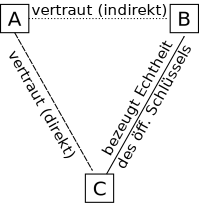
\includegraphics[width=0.5\textheight]{images/vertrauen.pdf}
  %TODO: überarbeiten
\end{center}
\end{frame}

\begin{frame}{Wie stellt man Vertrauen in öffentliche Schlüssel her?}
  \begin{itemize}
    \item S/MIME -- Hierarchischer Vertrauensansatz
    \begin{itemize}
      \item hier nicht behandelt
    \end{itemize}
    \item OpenPGP -- Dezentraler Vertrauensansatz
    \begin{itemize}
      \item jeder kann festlegen, wem er vertraut
      \begin{itemize}
        \item er kann die Echtheit eines Schlüssels\\ z.B. bei einem persönlichen Treffen überprüfen
      \end{itemize}
      \item jeder \emph{kann} sein Vertrauensnetz veröffentlichen (Web-of-Trust)
      \begin{itemize}
        \item Vorteil: Man kann ``Freunden von Freunden'' vertrauen
        \item Nachteil: Beziehungen zwischen Menschen öffentlich\\ Aber: Facebook sagt da viel mehr aus
      \end{itemize}
      %\item wird hier behandelt
    \end{itemize}
  \end{itemize}
\end{frame}

\begin{frame}{Welche Software benötigt man?}
  \begin{block}{OpenPGP Backend}
    Macht die eigentliche Ver-/Entschlüsselung \& Signatur

    \vspace{1ex}
    \begin{tabular}{cccc}
      Linux:            & Windows: & Android:     & Mac:\\
      \emph{schon dabei} & GPG4Win  & OpenKeychain & GPGTools\footnote{kommerziell}\\
    \end{tabular}
  \end{block}
  \begin{block}{Plug-In fürs Mailprogramm}
    Grafische Oberfläche, leichtere Schlüsselverwaltung, etc.

    \vspace{1ex}
    \begin{tabular}{cccc}
      Thunderbird: & Outlook: & K9-Mail:            & Apple Mail:\\
      Enigmail     & GPG4Win  & \emph{integriert} & GPGTools\\
    \end{tabular}
  \end{block}
\end{frame}

\endinput
